\documentclass{standalone}
\usepackage{tikz}
\usetikzlibrary{patterns, positioning}

\begin{document}
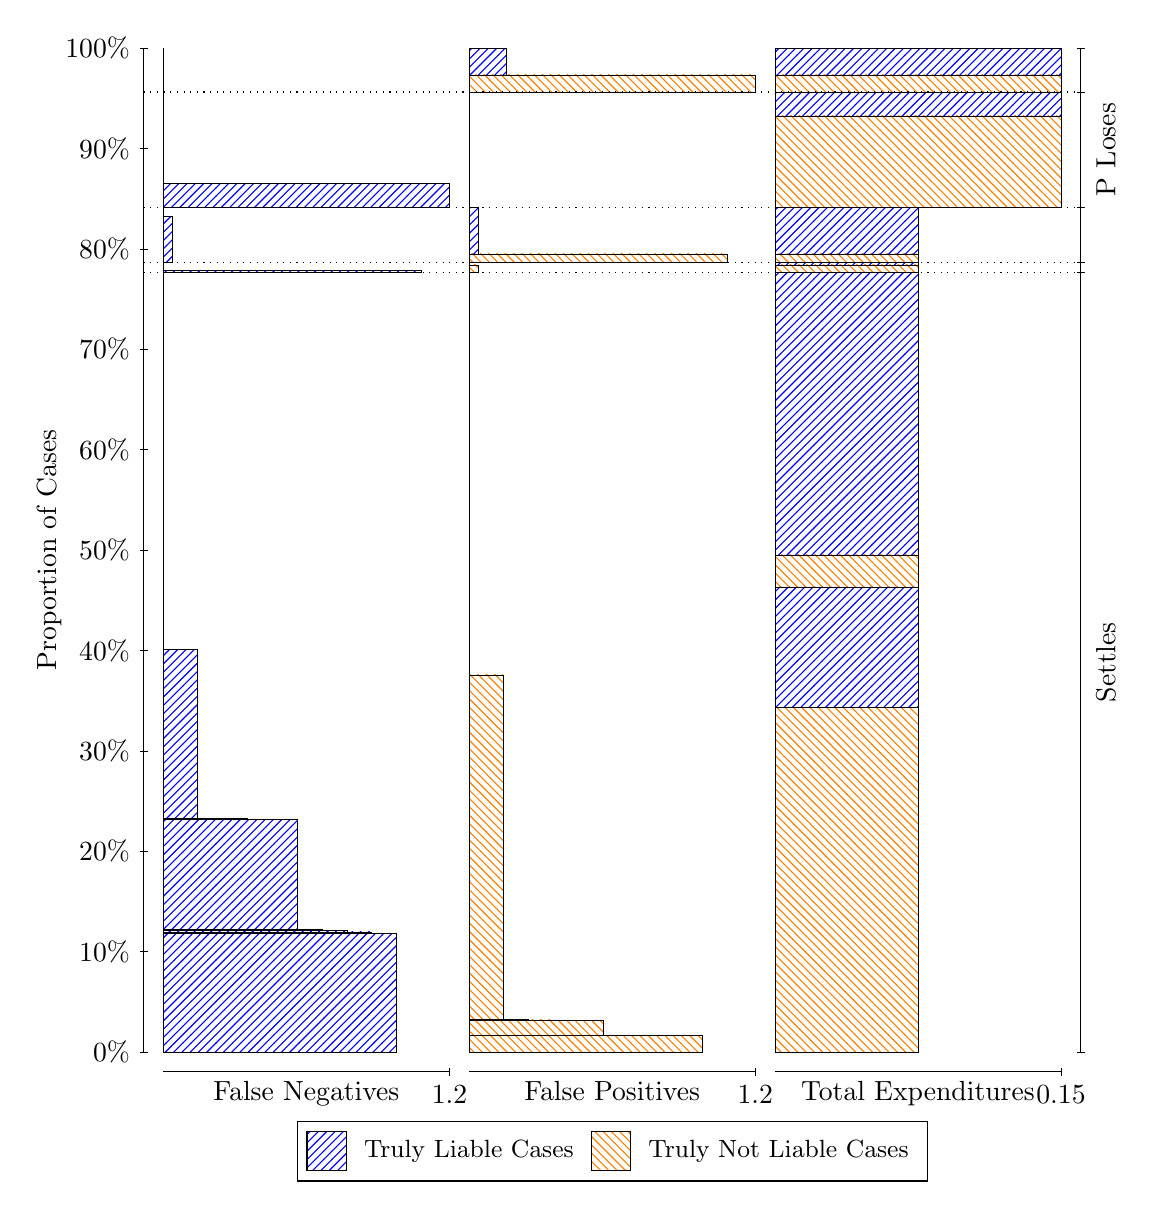
\begin{tikzpicture}
\draw[black, very thin] (1.5,1.75) -- (1.5,14.5);
\node[rotate=90, anchor=center] at (0.3, 8.125) {Proportion of Cases};
\draw[black, very thin] (1.45,1.75) -- (1.55,1.75);
\node[anchor=east] at (1.45, 1.75) {0\%};
\draw[black, very thin] (1.45,3.025) -- (1.55,3.025);
\node[anchor=east] at (1.45, 3.025) {10\%};
\draw[black, very thin] (1.45,4.3) -- (1.55,4.3);
\node[anchor=east] at (1.45, 4.3) {20\%};
\draw[black, very thin] (1.45,5.575) -- (1.55,5.575);
\node[anchor=east] at (1.45, 5.575) {30\%};
\draw[black, very thin] (1.45,6.85) -- (1.55,6.85);
\node[anchor=east] at (1.45, 6.85) {40\%};
\draw[black, very thin] (1.45,8.125) -- (1.55,8.125);
\node[anchor=east] at (1.45, 8.125) {50\%};
\draw[black, very thin] (1.45,9.4) -- (1.55,9.4);
\node[anchor=east] at (1.45, 9.4) {60\%};
\draw[black, very thin] (1.45,10.675) -- (1.55,10.675);
\node[anchor=east] at (1.45, 10.675) {70\%};
\draw[black, very thin] (1.45,11.95) -- (1.55,11.95);
\node[anchor=east] at (1.45, 11.95) {80\%};
\draw[black, very thin] (1.45,13.225) -- (1.55,13.225);
\node[anchor=east] at (1.45, 13.225) {90\%};
\draw[black, very thin] (1.45,14.5) -- (1.55,14.5);
\node[anchor=east] at (1.45, 14.5) {100\%};

\draw[black, very thin] (13.4,1.75) -- (13.4,14.5);
\draw[black, very thin] (13.35,1.75) -- (13.45,1.75);
\node[anchor=west] at (13.35, 1.75) {};
\draw[black, very thin] (13.35,11.65) -- (13.45,11.65);
\node[anchor=west] at (13.35, 11.65) {};
\draw[black, very thin] (13.35,11.776) -- (13.45,11.776);
\node[anchor=west] at (13.35, 11.776) {};
\draw[black, very thin] (13.35,12.478) -- (13.45,12.478);
\node[anchor=west] at (13.35, 12.478) {};
\draw[black, very thin] (13.35,13.941) -- (13.45,13.941);
\node[anchor=west] at (13.35, 13.941) {};
\draw[black, very thin] (13.35,14.5) -- (13.45,14.5);
\node[anchor=west] at (13.35, 14.5) {};

\draw[black, very thin, pattern color=blue, pattern=north east lines] (1.75,1.75) rectangle (4.712,3.2609);
\draw[black, very thin, pattern color=blue, pattern=north east lines] (1.75,3.2609) rectangle (4.396,3.2763);
\draw[black, very thin, pattern color=blue, pattern=north east lines] (1.75,3.2763) rectangle (4.0801,3.2919);
\draw[black, very thin, pattern color=blue, pattern=north east lines] (1.75,3.2919) rectangle (3.7641,3.3079);
\draw[black, very thin, pattern color=blue, pattern=north east lines] (1.75,3.3079) rectangle (3.4482,4.6995);
\draw[black, very thin, pattern color=blue, pattern=north east lines] (1.75,4.6995) rectangle (3.1322,4.7065);
\draw[black, very thin, pattern color=blue, pattern=north east lines] (1.75,4.7065) rectangle (2.8163,4.7136);
\draw[black, very thin, pattern color=blue, pattern=north east lines] (1.75,4.7136) rectangle (2.5004,4.7205);
\draw[black, very thin, pattern color=blue, pattern=north east lines] (1.75,4.7205) rectangle (2.1844,6.8625);
\draw[black, very thin, pattern color=orange, pattern=north west lines] (1.75,6.8625) rectangle (1.75,11.65);
\draw[black, very thin, pattern color=blue, pattern=north east lines] (1.75,11.65) rectangle (5.0279,11.679);
\draw[black, very thin, pattern color=orange, pattern=north west lines] (1.75,11.679) rectangle (1.75,11.776);
\draw[black, very thin, pattern color=blue, pattern=north east lines] (1.75,11.776) rectangle (1.8685,12.366);
\draw[black, very thin, pattern color=orange, pattern=north west lines] (1.75,12.366) rectangle (1.75,12.478);
\draw[black, very thin, pattern color=blue, pattern=north east lines] (1.75,12.478) rectangle (5.3833,12.781);
\draw[black, very thin, pattern color=orange, pattern=north west lines] (1.75,12.781) rectangle (1.75,13.941);
\draw[black, very thin, pattern color=orange, pattern=north west lines] (1.75,13.941) rectangle (1.75,14.16);
\draw[black, very thin, pattern color=blue, pattern=north east lines] (1.75,14.16) rectangle (1.75,14.5);
\draw[black, very thin, pattern color=orange, pattern=north west lines] (5.6333,1.75) rectangle (8.5953,1.9597);
\draw[black, very thin, pattern color=orange, pattern=north west lines] (5.6333,1.9597) rectangle (8.2793,1.9607);
\draw[black, very thin, pattern color=orange, pattern=north west lines] (5.6333,1.9607) rectangle (7.9634,1.9617);
\draw[black, very thin, pattern color=orange, pattern=north west lines] (5.6333,1.9617) rectangle (7.6475,1.9627);
\draw[black, very thin, pattern color=orange, pattern=north west lines] (5.6333,1.9627) rectangle (7.3315,2.1519);
\draw[black, very thin, pattern color=orange, pattern=north west lines] (5.6333,2.1519) rectangle (7.0156,2.1519);
\draw[black, very thin, pattern color=orange, pattern=north west lines] (5.6333,2.1519) rectangle (7.0156,2.1545);
\draw[black, very thin, pattern color=orange, pattern=north west lines] (5.6333,2.1545) rectangle (6.6996,2.157);
\draw[black, very thin, pattern color=orange, pattern=north west lines] (5.6333,2.157) rectangle (6.3837,2.1594);
\draw[black, very thin, pattern color=orange, pattern=north west lines] (5.6333,2.1594) rectangle (6.0678,6.5379);
\draw[black, very thin, pattern color=blue, pattern=north east lines] (5.6333,6.5379) rectangle (5.6333,11.65);
\draw[black, very thin, pattern color=orange, pattern=north west lines] (5.6333,11.65) rectangle (5.7518,11.747);
\draw[black, very thin, pattern color=blue, pattern=north east lines] (5.6333,11.747) rectangle (5.6333,11.776);
\draw[black, very thin, pattern color=orange, pattern=north west lines] (5.6333,11.776) rectangle (8.9112,11.887);
\draw[black, very thin, pattern color=blue, pattern=north east lines] (5.6333,11.887) rectangle (5.7518,12.478);
\draw[black, very thin, pattern color=orange, pattern=north west lines] (5.6333,12.478) rectangle (5.6333,13.639);
\draw[black, very thin, pattern color=blue, pattern=north east lines] (5.6333,13.639) rectangle (5.6333,13.941);
\draw[black, very thin, pattern color=orange, pattern=north west lines] (5.6333,13.941) rectangle (9.2667,14.16);
\draw[black, very thin, pattern color=blue, pattern=north east lines] (5.6333,14.16) rectangle (6.1072,14.5);
\draw[black, very thin, pattern color=orange, pattern=north west lines] (9.5167,1.75) rectangle (11.333,6.1309);
\draw[black, very thin, pattern color=blue, pattern=north east lines] (9.5167,6.1309) rectangle (11.333,7.6571);
\draw[black, very thin, pattern color=orange, pattern=north west lines] (9.5167,7.6571) rectangle (11.333,8.0642);
\draw[black, very thin, pattern color=blue, pattern=north east lines] (9.5167,8.0642) rectangle (11.333,11.65);
\draw[black, very thin, pattern color=orange, pattern=north west lines] (9.5167,11.65) rectangle (11.333,11.747);
\draw[black, very thin, pattern color=blue, pattern=north east lines] (9.5167,11.747) rectangle (11.333,11.776);
\draw[black, very thin, pattern color=orange, pattern=north west lines] (9.5167,11.776) rectangle (11.333,11.887);
\draw[black, very thin, pattern color=blue, pattern=north east lines] (9.5167,11.887) rectangle (11.333,12.478);
\draw[black, very thin, pattern color=orange, pattern=north west lines] (9.5167,12.478) rectangle (13.15,13.639);
\draw[black, very thin, pattern color=blue, pattern=north east lines] (9.5167,13.639) rectangle (13.15,13.941);
\draw[black, very thin, pattern color=orange, pattern=north west lines] (9.5167,13.941) rectangle (13.15,14.16);
\draw[black, very thin, pattern color=blue, pattern=north east lines] (9.5167,14.16) rectangle (13.15,14.5);
\draw[black, dotted] (1.5,11.65) -- (13.4,11.65);
\draw[black, dotted] (1.5,11.776) -- (13.4,11.776);
\draw[black, dotted] (1.5,12.478) -- (13.4,12.478);
\draw[black, dotted] (1.5,13.941) -- (13.4,13.941);
\draw[black, very thin] (1.75,1.5) -- (5.3833,1.5);
\node[anchor=north] at (3.5667, 1.5) {False Negatives};
\draw[black, very thin] (5.3833,1.45) -- (5.3833,1.55);
\node[anchor=north] at (5.3833, 1.45) {1.2};

\draw[black, very thin] (5.6333,1.5) -- (9.2667,1.5);
\node[anchor=north] at (7.45, 1.5) {False Positives};
\draw[black, very thin] (9.2667,1.45) -- (9.2667,1.55);
\node[anchor=north] at (9.2667, 1.45) {1.2};

\draw[black, very thin] (9.5167,1.5) -- (13.15,1.5);
\node[anchor=north] at (11.333, 1.5) {Total Expenditures};
\draw[black, very thin] (13.15,1.45) -- (13.15,1.55);
\node[anchor=north] at (13.15, 1.45) {0.15};

\node[black, centered, rotate=90] at (13.72, 6.7002) {Settles};


\node[black, centered, rotate=90] at (13.72, 13.21) {P Loses};


\draw (7.449999999999999,1.5) node[draw=none] (baseCoordinate) {};
\begin{scope}[align=center]
        \matrix[scale=0.5, draw=black, below=0.5cm of baseCoordinate, nodes={draw}, column sep=0.1cm]{
            \node[rectangle, draw, minimum width=0.5cm, minimum height=0.5cm, pattern=north east lines, pattern color=blue] {}; &
            \node[draw=none, font=\small] (B) {Truly Liable Cases}; &
            \node[rectangle, draw, minimum width=0.5cm, minimum height=0.5cm, pattern=north west lines, pattern color=orange] {}; &
            \node[draw=none, font=\small] (B) {Truly Not Liable Cases}; \\
            };
\end{scope}

\end{tikzpicture}
\end{document}